\documentclass[1p]{elsarticle_modified}
%\bibliographystyle{elsarticle-num}

%\usepackage[colorlinks]{hyperref}
%\usepackage{abbrmath_seonhwa} %\Abb, \Ascr, \Acal ,\Abf, \Afrak
\usepackage{amsfonts}
\usepackage{amssymb}
\usepackage{amsmath}
\usepackage{amsthm}
\usepackage{scalefnt}
\usepackage{amsbsy}
\usepackage{kotex}
\usepackage{caption}
\usepackage{subfig}
\usepackage{color}
\usepackage{graphicx}
\usepackage{xcolor} %% white, black, red, green, blue, cyan, magenta, yellow
\usepackage{float}
\usepackage{setspace}
\usepackage{hyperref}

\usepackage{tikz}
\usetikzlibrary{arrows}

\usepackage{multirow}
\usepackage{array} % fixed length table
\usepackage{hhline}

%%%%%%%%%%%%%%%%%%%%%
\makeatletter
\renewcommand*\env@matrix[1][\arraystretch]{%
	\edef\arraystretch{#1}%
	\hskip -\arraycolsep
	\let\@ifnextchar\new@ifnextchar
	\array{*\c@MaxMatrixCols c}}
\makeatother %https://tex.stackexchange.com/questions/14071/how-can-i-increase-the-line-spacing-in-a-matrix
%%%%%%%%%%%%%%%

\usepackage[normalem]{ulem}

\newcommand{\msout}[1]{\ifmmode\text{\sout{\ensuremath{#1}}}\else\sout{#1}\fi}
%SOURCE: \msout is \stkout macro in https://tex.stackexchange.com/questions/20609/strikeout-in-math-mode

\newcommand{\cancel}[1]{
	\ifmmode
	{\color{red}\msout{#1}}
	\else
	{\color{red}\sout{#1}}
	\fi
}

\newcommand{\add}[1]{
	{\color{blue}\uwave{#1}}
}

\newcommand{\replace}[2]{
	\ifmmode
	{\color{red}\msout{#1}}{\color{blue}\uwave{#2}}
	\else
	{\color{red}\sout{#1}}{\color{blue}\uwave{#2}}
	\fi
}

\newcommand{\Sol}{\mathcal{S}} %segment
\newcommand{\D}{D} %diagram
\newcommand{\A}{\mathcal{A}} %arc


%%%%%%%%%%%%%%%%%%%%%%%%%%%%%5 test

\def\sl{\operatorname{\textup{SL}}(2,\Cbb)}
\def\psl{\operatorname{\textup{PSL}}(2,\Cbb)}
\def\quan{\mkern 1mu \triangleright \mkern 1mu}

\theoremstyle{definition}
\newtheorem{thm}{Theorem}[section]
\newtheorem{prop}[thm]{Proposition}
\newtheorem{lem}[thm]{Lemma}
\newtheorem{ques}[thm]{Question}
\newtheorem{cor}[thm]{Corollary}
\newtheorem{defn}[thm]{Definition}
\newtheorem{exam}[thm]{Example}
\newtheorem{rmk}[thm]{Remark}
\newtheorem{alg}[thm]{Algorithm}

\newcommand{\I}{\sqrt{-1}}
\begin{document}

%\begin{frontmatter}
%
%\title{Boundary parabolic representations of knots up to 8 crossings}
%
%%% Group authors per affiliation:
%\author{Yunhi Cho} 
%\address{Department of Mathematics, University of Seoul, Seoul, Korea}
%\ead{yhcho@uos.ac.kr}
%
%
%\author{Seonhwa Kim} %\fnref{s_kim}}
%\address{Center for Geometry and Physics, Institute for Basic Science, Pohang, 37673, Korea}
%\ead{ryeona17@ibs.re.kr}
%
%\author{Hyuk Kim}
%\address{Department of Mathematical Sciences, Seoul National University, Seoul 08826, Korea}
%\ead{hyukkim@snu.ac.kr}
%
%\author{Seokbeom Yoon}
%\address{Department of Mathematical Sciences, Seoul National University, Seoul, 08826,  Korea}
%\ead{sbyoon15@snu.ac.kr}
%
%\begin{abstract}
%We find all boundary parabolic representation of knots up to 8 crossings.
%
%\end{abstract}
%\begin{keyword}
%    \MSC[2010] 57M25 
%\end{keyword}
%
%\end{frontmatter}

%\linenumbers
%\tableofcontents
%
\newcommand\colored[1]{\textcolor{white}{\rule[-0.35ex]{0.8em}{1.4ex}}\kern-0.8em\color{red} #1}%
%\newcommand\colored[1]{\textcolor{white}{ #1}\kern-2.17ex	\textcolor{white}{ #1}\kern-1.81ex	\textcolor{white}{ #1}\kern-2.15ex\color{red}#1	}

{\Large $\underline{11n_{85}~(K11n_{85})}$}

\setlength{\tabcolsep}{10pt}
\renewcommand{\arraystretch}{1.6}
\vspace{1cm}\begin{tabular}{m{100pt}>{\centering\arraybackslash}m{274pt}}
\multirow{5}{120pt}{
	\centering
	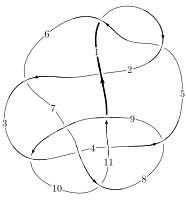
\includegraphics[width=112pt]{../../../GIT/diagram.site/Diagrams/png/701_11n_85.png}\\
\ \ \ A knot diagram\footnotemark}&
\allowdisplaybreaks
\textbf{Linearized knot diagam} \\
\cline{2-2}
 &
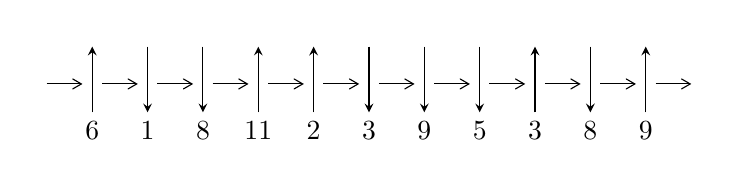
\begin{tikzpicture}[x=20pt, y=17pt]
	% nodes
	\node (C0) at (0, 0) {};
	\node (C1) at (1, 0) {};
	\node (C1U) at (1, +1) {};
	\node (C1D) at (1, -1) {6};

	\node (C2) at (2, 0) {};
	\node (C2U) at (2, +1) {};
	\node (C2D) at (2, -1) {1};

	\node (C3) at (3, 0) {};
	\node (C3U) at (3, +1) {};
	\node (C3D) at (3, -1) {8};

	\node (C4) at (4, 0) {};
	\node (C4U) at (4, +1) {};
	\node (C4D) at (4, -1) {11};

	\node (C5) at (5, 0) {};
	\node (C5U) at (5, +1) {};
	\node (C5D) at (5, -1) {2};

	\node (C6) at (6, 0) {};
	\node (C6U) at (6, +1) {};
	\node (C6D) at (6, -1) {3};

	\node (C7) at (7, 0) {};
	\node (C7U) at (7, +1) {};
	\node (C7D) at (7, -1) {9};

	\node (C8) at (8, 0) {};
	\node (C8U) at (8, +1) {};
	\node (C8D) at (8, -1) {5};

	\node (C9) at (9, 0) {};
	\node (C9U) at (9, +1) {};
	\node (C9D) at (9, -1) {3};

	\node (C10) at (10, 0) {};
	\node (C10U) at (10, +1) {};
	\node (C10D) at (10, -1) {8};

	\node (C11) at (11, 0) {};
	\node (C11U) at (11, +1) {};
	\node (C11D) at (11, -1) {9};
	\node (C12) at (12, 0) {};

	% arrows
	\draw[->,>={angle 60}]
	(C0) edge (C1) (C1) edge (C2) (C2) edge (C3) (C3) edge (C4) (C4) edge (C5) (C5) edge (C6) (C6) edge (C7) (C7) edge (C8) (C8) edge (C9) (C9) edge (C10) (C10) edge (C11) (C11) edge (C12) ;	\draw[->,>=stealth]
	(C1D) edge (C1U) (C2U) edge (C2D) (C3U) edge (C3D) (C4D) edge (C4U) (C5D) edge (C5U) (C6U) edge (C6D) (C7U) edge (C7D) (C8U) edge (C8D) (C9D) edge (C9U) (C10U) edge (C10D) (C11D) edge (C11U) ;
	\end{tikzpicture} \\
\hhline{~~} \\& 
\textbf{Solving Sequence} \\ \cline{2-2} 
 &
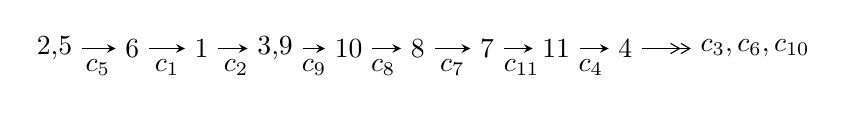
\begin{tikzpicture}[x=25pt, y=7pt]
	% node
	\node (A0) at (-1/8, 0) {2,5};
	\node (A1) at (1, 0) {6};
	\node (A2) at (2, 0) {1};
	\node (A3) at (49/16, 0) {3,9};
	\node (A4) at (33/8, 0) {10};
	\node (A5) at (41/8, 0) {8};
	\node (A6) at (49/8, 0) {7};
	\node (A7) at (57/8, 0) {11};
	\node (A8) at (65/8, 0) {4};
	\node (C1) at (1/2, -1) {$c_{5}$};
	\node (C2) at (3/2, -1) {$c_{1}$};
	\node (C3) at (5/2, -1) {$c_{2}$};
	\node (C4) at (29/8, -1) {$c_{9}$};
	\node (C5) at (37/8, -1) {$c_{8}$};
	\node (C6) at (45/8, -1) {$c_{7}$};
	\node (C7) at (53/8, -1) {$c_{11}$};
	\node (C8) at (61/8, -1) {$c_{4}$};
	\node (A9) at (10, 0) {$c_{3},c_{6},c_{10}$};

	% edge
	\draw[->,>=stealth]	
	(A0) edge (A1) (A1) edge (A2) (A2) edge (A3) (A3) edge (A4) (A4) edge (A5) (A5) edge (A6) (A6) edge (A7) (A7) edge (A8) ;
	\draw[->>,>={angle 60}]	
	(A8) edge (A9);
\end{tikzpicture} \\ 

\end{tabular} \\

\footnotetext{
The image of knot diagram is generated by the software ``\textbf{Draw programme}" developed by Andrew Bartholomew(\url{http://www.layer8.co.uk/maths/draw/index.htm\#Running-draw}), where we modified some parts for our purpose(\url{https://github.com/CATsTAILs/LinksPainter}).
}\phantom \\ \newline 
\centering \textbf{Ideals for irreducible components\footnotemark of $X_{\text{par}}$} 
 
\begin{align*}
I^u_{1}&=\langle 
-2 u^{22}-2 u^{21}+\cdots+4 b-2,\;2 u^{22}+u^{21}+\cdots+4 a-2,\;u^{23}+2 u^{22}+\cdots+4 u+2\rangle \\
I^u_{2}&=\langle 
b+1,\;u^3+2 u^2+2 a+4,\;u^4+2 u^2+2\rangle \\
I^u_{3}&=\langle 
- a^2 u+2 b+a-2,\;a^3+2 a^2 u- a u+2 a+2,\;u^2- u+1\rangle \\
\\
I^v_{1}&=\langle 
a,\;b-1,\;v-1\rangle \\
\end{align*}
\raggedright * 4 irreducible components of $\dim_{\mathbb{C}}=0$, with total 34 representations.\\
\footnotetext{All coefficients of polynomials are rational numbers. But the coefficients are sometimes approximated in decimal forms when there is not enough margin.}
\newpage
\renewcommand{\arraystretch}{1}
\centering \section*{I. $I^u_{1}= \langle -2 u^{22}-2 u^{21}+\cdots+4 b-2,\;2 u^{22}+u^{21}+\cdots+4 a-2,\;u^{23}+2 u^{22}+\cdots+4 u+2 \rangle$}
\flushleft \textbf{(i) Arc colorings}\\
\begin{tabular}{m{7pt} m{180pt} m{7pt} m{180pt} }
\flushright $a_{2}=$&$\begin{pmatrix}0\\u\end{pmatrix}$ \\
\flushright $a_{5}=$&$\begin{pmatrix}1\\0\end{pmatrix}$ \\
\flushright $a_{6}=$&$\begin{pmatrix}1\\- u^2\end{pmatrix}$ \\
\flushright $a_{1}=$&$\begin{pmatrix}- u\\u^3+u\end{pmatrix}$ \\
\flushright $a_{3}=$&$\begin{pmatrix}- u^3\\u^5+u^3+u\end{pmatrix}$ \\
\flushright $a_{9}=$&$\begin{pmatrix}-\frac{1}{2} u^{22}-\frac{1}{4} u^{21}+\cdots-\frac{1}{2} u+\frac{1}{2}\\\frac{1}{2} u^{22}+\frac{1}{2} u^{21}+\cdots+\frac{1}{2} u+\frac{1}{2}\end{pmatrix}$ \\
\flushright $a_{10}=$&$\begin{pmatrix}-\frac{1}{4} u^{18}- u^{16}+\cdots+\frac{1}{2} u+\frac{1}{2}\\-\frac{1}{2} u^{13}-\frac{3}{2} u^{11}+\cdots- u^3- u\end{pmatrix}$ \\
\flushright $a_{8}=$&$\begin{pmatrix}\frac{1}{4} u^{21}+u^{19}+\cdots-\frac{1}{2} u^3+1\\\frac{1}{2} u^{22}+\frac{1}{2} u^{21}+\cdots+\frac{1}{2} u+\frac{1}{2}\end{pmatrix}$ \\
\flushright $a_{7}=$&$\begin{pmatrix}- u^6- u^4+1\\u^8+2 u^6+2 u^4\end{pmatrix}$ \\
\flushright $a_{11}=$&$\begin{pmatrix}\frac{1}{2} u^{22}+\frac{3}{4} u^{21}+\cdots-\frac{1}{2} u-\frac{1}{2}\\\frac{1}{2} u^{22}+\frac{1}{2} u^{21}+\cdots+\frac{3}{2} u+\frac{1}{2}\end{pmatrix}$ \\
\flushright $a_{4}=$&$\begin{pmatrix}-\frac{1}{4} u^{21}- u^{19}+\cdots-\frac{3}{2} u^3- u\\-\frac{1}{4} u^{21}-\frac{5}{4} u^{19}+\cdots+\frac{1}{2} u^2+\frac{1}{2} u\end{pmatrix}$\\ \flushright $a_{4}=$&$\begin{pmatrix}-\frac{1}{4} u^{21}- u^{19}+\cdots-\frac{3}{2} u^3- u\\-\frac{1}{4} u^{21}-\frac{5}{4} u^{19}+\cdots+\frac{1}{2} u^2+\frac{1}{2} u\end{pmatrix}$\\&\end{tabular}
\flushleft \textbf{(ii) Obstruction class $= -1$}\\~\\
\flushleft \textbf{(iii) Cusp Shapes $= 2 u^{22}+4 u^{21}+10 u^{20}+16 u^{19}+24 u^{18}+34 u^{17}+30 u^{16}+40 u^{15}+16 u^{14}+30 u^{13}+32 u^{11}+8 u^{10}+46 u^9+14 u^8+42 u^7-8 u^6+2 u^5-24 u^4+2 u^3+4 u^2+10 u$}\\~\\
\newpage\renewcommand{\arraystretch}{1}
\flushleft \textbf{(iv) u-Polynomials at the component}\newline \\
\begin{tabular}{m{50pt}|m{274pt}}
Crossings & \hspace{64pt}u-Polynomials at each crossing \\
\hline $$\begin{aligned}c_{1},c_{5}\end{aligned}$$&$\begin{aligned}
&u^{23}+2 u^{22}+\cdots+4 u+2
\end{aligned}$\\
\hline $$\begin{aligned}c_{2}\end{aligned}$$&$\begin{aligned}
&u^{23}+10 u^{22}+\cdots+8 u-4
\end{aligned}$\\
\hline $$\begin{aligned}c_{3}\end{aligned}$$&$\begin{aligned}
&u^{23}+27 u^{21}+\cdots-7 u+1
\end{aligned}$\\
\hline $$\begin{aligned}c_{4},c_{9}\end{aligned}$$&$\begin{aligned}
&u^{23}-2 u^{22}+\cdots+9 u+1
\end{aligned}$\\
\hline $$\begin{aligned}c_{6}\end{aligned}$$&$\begin{aligned}
&u^{23}-2 u^{22}+\cdots-88 u+16
\end{aligned}$\\
\hline $$\begin{aligned}c_{7}\end{aligned}$$&$\begin{aligned}
&u^{23}+2 u^{22}+\cdots-11 u+1
\end{aligned}$\\
\hline $$\begin{aligned}c_{8}\end{aligned}$$&$\begin{aligned}
&u^{23}+2 u^{22}+\cdots-3 u+1
\end{aligned}$\\
\hline $$\begin{aligned}c_{10}\end{aligned}$$&$\begin{aligned}
&u^{23}-5 u^{22}+\cdots+128 u+1706
\end{aligned}$\\
\hline $$\begin{aligned}c_{11}\end{aligned}$$&$\begin{aligned}
&u^{23}+8 u^{22}+\cdots+1035 u+297
\end{aligned}$\\
\hline
\end{tabular}\\~\\
\newpage\renewcommand{\arraystretch}{1}
\flushleft \textbf{(v) Riley Polynomials at the component}\newline \\
\begin{tabular}{m{50pt}|m{274pt}}
Crossings & \hspace{64pt}Riley Polynomials at each crossing \\
\hline $$\begin{aligned}c_{1},c_{5}\end{aligned}$$&$\begin{aligned}
&y^{23}+10 y^{22}+\cdots+8 y-4
\end{aligned}$\\
\hline $$\begin{aligned}c_{2}\end{aligned}$$&$\begin{aligned}
&y^{23}+6 y^{22}+\cdots+160 y-16
\end{aligned}$\\
\hline $$\begin{aligned}c_{3}\end{aligned}$$&$\begin{aligned}
&y^{23}+54 y^{22}+\cdots+25 y-1
\end{aligned}$\\
\hline $$\begin{aligned}c_{4},c_{9}\end{aligned}$$&$\begin{aligned}
&y^{23}-34 y^{22}+\cdots-27 y-1
\end{aligned}$\\
\hline $$\begin{aligned}c_{6}\end{aligned}$$&$\begin{aligned}
&y^{23}+2 y^{22}+\cdots+960 y-256
\end{aligned}$\\
\hline $$\begin{aligned}c_{7}\end{aligned}$$&$\begin{aligned}
&y^{23}+46 y^{22}+\cdots-135 y-1
\end{aligned}$\\
\hline $$\begin{aligned}c_{8}\end{aligned}$$&$\begin{aligned}
&y^{23}-2 y^{22}+\cdots-11 y-1
\end{aligned}$\\
\hline $$\begin{aligned}c_{10}\end{aligned}$$&$\begin{aligned}
&y^{23}+41 y^{22}+\cdots-12287288 y-2910436
\end{aligned}$\\
\hline $$\begin{aligned}c_{11}\end{aligned}$$&$\begin{aligned}
&y^{23}-26 y^{22}+\cdots+935793 y-88209
\end{aligned}$\\
\hline
\end{tabular}\\~\\
\newpage\flushleft \textbf{(vi) Complex Volumes and Cusp Shapes}
$$\begin{array}{c|c|c}  
\text{Solutions to }I^u_{1}& \I (\text{vol} + \sqrt{-1}CS) & \text{Cusp shape}\\
 \hline 
\begin{aligned}
u &= \phantom{-}0.887093 + 0.448454 I \\
a &= \phantom{-}0.492271 + 1.285580 I \\
b &= -1.14839 - 1.01565 I\end{aligned}
 & \phantom{-}11.55830 - 6.04378 I & \phantom{-}2.90457 + 2.40956 I \\ \hline\begin{aligned}
u &= \phantom{-}0.887093 - 0.448454 I \\
a &= \phantom{-}0.492271 - 1.285580 I \\
b &= -1.14839 + 1.01565 I\end{aligned}
 & \phantom{-}11.55830 + 6.04378 I & \phantom{-}2.90457 - 2.40956 I \\ \hline\begin{aligned}
u &= -0.865908 + 0.562605 I \\
a &= \phantom{-}0.29789 + 1.55245 I \\
b &= -0.94225 - 1.16788 I\end{aligned}
 & \phantom{-}12.26940 - 1.86843 I & \phantom{-}3.51927 + 2.09858 I \\ \hline\begin{aligned}
u &= -0.865908 - 0.562605 I \\
a &= \phantom{-}0.29789 - 1.55245 I \\
b &= -0.94225 + 1.16788 I\end{aligned}
 & \phantom{-}12.26940 + 1.86843 I & \phantom{-}3.51927 - 2.09858 I \\ \hline\begin{aligned}
u &= -0.126252 + 0.927958 I \\
a &= \phantom{-}0.472434 + 0.373694 I \\
b &= \phantom{-}0.816023 - 0.401741 I\end{aligned}
 & -1.83455 + 1.28121 I & -6.39377 - 3.70883 I \\ \hline\begin{aligned}
u &= -0.126252 - 0.927958 I \\
a &= \phantom{-}0.472434 - 0.373694 I \\
b &= \phantom{-}0.816023 + 0.401741 I\end{aligned}
 & -1.83455 - 1.28121 I & -6.39377 + 3.70883 I \\ \hline\begin{aligned}
u &= -0.687410 + 0.551797 I \\
a &= \phantom{-}0.93433 - 1.33726 I \\
b &= -0.566101 + 0.784858 I\end{aligned}
 & \phantom{-}2.63493 + 2.12803 I & \phantom{-}3.22069 - 2.55962 I \\ \hline\begin{aligned}
u &= -0.687410 - 0.551797 I \\
a &= \phantom{-}0.93433 + 1.33726 I \\
b &= -0.566101 - 0.784858 I\end{aligned}
 & \phantom{-}2.63493 - 2.12803 I & \phantom{-}3.22069 + 2.55962 I \\ \hline\begin{aligned}
u &= -0.439313 + 1.087580 I \\
a &= -1.12704 + 1.03997 I \\
b &= -1.028740 - 0.075248 I\end{aligned}
 & -4.16811 - 3.61856 I & -9.97032 + 4.29272 I \\ \hline\begin{aligned}
u &= -0.439313 - 1.087580 I \\
a &= -1.12704 - 1.03997 I \\
b &= -1.028740 + 0.075248 I\end{aligned}
 & -4.16811 + 3.61856 I & -9.97032 - 4.29272 I\\
 \hline 
 \end{array}$$\newpage$$\begin{array}{c|c|c}  
\text{Solutions to }I^u_{1}& \I (\text{vol} + \sqrt{-1}CS) & \text{Cusp shape}\\
 \hline 
\begin{aligned}
u &= -0.611535 + 1.029680 I \\
a &= \phantom{-}0.57884 - 1.78933 I \\
b &= \phantom{-}0.744103 + 0.840632 I\end{aligned}
 & \phantom{-}1.22653 - 7.16348 I & -0.15345 + 7.54828 I \\ \hline\begin{aligned}
u &= -0.611535 - 1.029680 I \\
a &= \phantom{-}0.57884 + 1.78933 I \\
b &= \phantom{-}0.744103 - 0.840632 I\end{aligned}
 & \phantom{-}1.22653 + 7.16348 I & -0.15345 - 7.54828 I \\ \hline\begin{aligned}
u &= \phantom{-}0.470162 + 1.125140 I \\
a &= -1.139790 - 0.221923 I \\
b &= -0.174623 + 0.267387 I\end{aligned}
 & -0.75408 + 3.78076 I & \phantom{-}1.64329 - 3.83078 I \\ \hline\begin{aligned}
u &= \phantom{-}0.470162 - 1.125140 I \\
a &= -1.139790 + 0.221923 I \\
b &= -0.174623 - 0.267387 I\end{aligned}
 & -0.75408 - 3.78076 I & \phantom{-}1.64329 + 3.83078 I \\ \hline\begin{aligned}
u &= \phantom{-}0.066964 + 1.228960 I \\
a &= \phantom{-}0.900031 + 0.128011 I \\
b &= \phantom{-}0.988654 + 0.944921 I\end{aligned}
 & \phantom{-}5.54974 - 3.50228 I & -1.93120 + 2.15966 I \\ \hline\begin{aligned}
u &= \phantom{-}0.066964 - 1.228960 I \\
a &= \phantom{-}0.900031 - 0.128011 I \\
b &= \phantom{-}0.988654 - 0.944921 I\end{aligned}
 & \phantom{-}5.54974 + 3.50228 I & -1.93120 - 2.15966 I \\ \hline\begin{aligned}
u &= -0.694097 + 1.072020 I \\
a &= -1.125380 + 0.108515 I \\
b &= \phantom{-}0.83601 - 1.20931 I\end{aligned}
 & \phantom{-}10.72870 - 3.91001 I & \phantom{-}1.79235 + 2.50229 I \\ \hline\begin{aligned}
u &= -0.694097 - 1.072020 I \\
a &= -1.125380 - 0.108515 I \\
b &= \phantom{-}0.83601 + 1.20931 I\end{aligned}
 & \phantom{-}10.72870 + 3.91001 I & \phantom{-}1.79235 - 2.50229 I \\ \hline\begin{aligned}
u &= \phantom{-}0.652491 + 1.132530 I \\
a &= \phantom{-}1.13140 + 1.85064 I \\
b &= \phantom{-}1.20493 - 0.95597 I\end{aligned}
 & \phantom{-}9.4833 + 11.7267 I & \phantom{-}0.34491 - 6.55767 I \\ \hline\begin{aligned}
u &= \phantom{-}0.652491 - 1.132530 I \\
a &= \phantom{-}1.13140 - 1.85064 I \\
b &= \phantom{-}1.20493 + 0.95597 I\end{aligned}
 & \phantom{-}9.4833 - 11.7267 I & \phantom{-}0.34491 + 6.55767 I\\
 \hline 
 \end{array}$$\newpage$$\begin{array}{c|c|c}  
\text{Solutions to }I^u_{1}& \I (\text{vol} + \sqrt{-1}CS) & \text{Cusp shape}\\
 \hline 
\begin{aligned}
u &= \phantom{-}0.601530 + 0.285314 I \\
a &= \phantom{-}1.041030 - 0.706848 I \\
b &= -0.179556 + 0.418301 I\end{aligned}
 & \phantom{-}1.74084 + 0.44680 I & \phantom{-}5.28361 - 1.38333 I \\ \hline\begin{aligned}
u &= \phantom{-}0.601530 - 0.285314 I \\
a &= \phantom{-}1.041030 + 0.706848 I \\
b &= -0.179556 - 0.418301 I\end{aligned}
 & \phantom{-}1.74084 - 0.44680 I & \phantom{-}5.28361 + 1.38333 I \\ \hline\begin{aligned}
u &= -0.507450\phantom{ +0.000000I} \\
a &= \phantom{-}0.0879637\phantom{ +0.000000I} \\
b &= \phantom{-}0.899884\phantom{ +0.000000I}\end{aligned}
 & -1.46388\phantom{ +0.000000I} & -6.51990\phantom{ +0.000000I}\\
 \hline 
 \end{array}$$\newpage\newpage\renewcommand{\arraystretch}{1}
\centering \section*{II. $I^u_{2}= \langle b+1,\;u^3+2 u^2+2 a+4,\;u^4+2 u^2+2 \rangle$}
\flushleft \textbf{(i) Arc colorings}\\
\begin{tabular}{m{7pt} m{180pt} m{7pt} m{180pt} }
\flushright $a_{2}=$&$\begin{pmatrix}0\\u\end{pmatrix}$ \\
\flushright $a_{5}=$&$\begin{pmatrix}1\\0\end{pmatrix}$ \\
\flushright $a_{6}=$&$\begin{pmatrix}1\\- u^2\end{pmatrix}$ \\
\flushright $a_{1}=$&$\begin{pmatrix}- u\\u^3+u\end{pmatrix}$ \\
\flushright $a_{3}=$&$\begin{pmatrix}- u^3\\- u^3- u\end{pmatrix}$ \\
\flushright $a_{9}=$&$\begin{pmatrix}-\frac{1}{2} u^3- u^2-2\\-1\end{pmatrix}$ \\
\flushright $a_{10}=$&$\begin{pmatrix}\frac{1}{2} u^3- u^2-2\\u^3+u-1\end{pmatrix}$ \\
\flushright $a_{8}=$&$\begin{pmatrix}-\frac{1}{2} u^3- u^2-3\\-1\end{pmatrix}$ \\
\flushright $a_{7}=$&$\begin{pmatrix}-1\\0\end{pmatrix}$ \\
\flushright $a_{11}=$&$\begin{pmatrix}-\frac{3}{2} u^3- u^2- u-3\\-1\end{pmatrix}$ \\
\flushright $a_{4}=$&$\begin{pmatrix}\frac{3}{2} u^3+u^2+u+4\\1\end{pmatrix}$\\ \flushright $a_{4}=$&$\begin{pmatrix}\frac{3}{2} u^3+u^2+u+4\\1\end{pmatrix}$\\&\end{tabular}
\flushleft \textbf{(ii) Obstruction class $= 1$}\\~\\
\flushleft \textbf{(iii) Cusp Shapes $= -4 u^2-8$}\\~\\
\newpage\renewcommand{\arraystretch}{1}
\flushleft \textbf{(iv) u-Polynomials at the component}\newline \\
\begin{tabular}{m{50pt}|m{274pt}}
Crossings & \hspace{64pt}u-Polynomials at each crossing \\
\hline $$\begin{aligned}c_{1},c_{5}\end{aligned}$$&$\begin{aligned}
&u^4+2 u^2+2
\end{aligned}$\\
\hline $$\begin{aligned}c_{2}\end{aligned}$$&$\begin{aligned}
&(u^2+2 u+2)^2
\end{aligned}$\\
\hline $$\begin{aligned}c_{3}\end{aligned}$$&$\begin{aligned}
&u^4+4 u^3+4 u^2+1
\end{aligned}$\\
\hline $$\begin{aligned}c_{4}\end{aligned}$$&$\begin{aligned}
&(u+1)^4
\end{aligned}$\\
\hline $$\begin{aligned}c_{6},c_{10}\end{aligned}$$&$\begin{aligned}
&u^4-2 u^2+2
\end{aligned}$\\
\hline $$\begin{aligned}c_{7},c_{8},c_{9}\end{aligned}$$&$\begin{aligned}
&(u-1)^4
\end{aligned}$\\
\hline $$\begin{aligned}c_{11}\end{aligned}$$&$\begin{aligned}
&u^4-4 u^3+4 u^2+1
\end{aligned}$\\
\hline
\end{tabular}\\~\\
\newpage\renewcommand{\arraystretch}{1}
\flushleft \textbf{(v) Riley Polynomials at the component}\newline \\
\begin{tabular}{m{50pt}|m{274pt}}
Crossings & \hspace{64pt}Riley Polynomials at each crossing \\
\hline $$\begin{aligned}c_{1},c_{5}\end{aligned}$$&$\begin{aligned}
&(y^2+2 y+2)^2
\end{aligned}$\\
\hline $$\begin{aligned}c_{2}\end{aligned}$$&$\begin{aligned}
&(y^2+4)^2
\end{aligned}$\\
\hline $$\begin{aligned}c_{3},c_{11}\end{aligned}$$&$\begin{aligned}
&y^4-8 y^3+18 y^2+8 y+1
\end{aligned}$\\
\hline $$\begin{aligned}c_{4},c_{7},c_{8}\\c_{9}\end{aligned}$$&$\begin{aligned}
&(y-1)^4
\end{aligned}$\\
\hline $$\begin{aligned}c_{6},c_{10}\end{aligned}$$&$\begin{aligned}
&(y^2-2 y+2)^2
\end{aligned}$\\
\hline
\end{tabular}\\~\\
\newpage\flushleft \textbf{(vi) Complex Volumes and Cusp Shapes}
$$\begin{array}{c|c|c}  
\text{Solutions to }I^u_{2}& \I (\text{vol} + \sqrt{-1}CS) & \text{Cusp shape}\\
 \hline 
\begin{aligned}
u &= \phantom{-}0.455090 + 1.098680 I \\
a &= -0.223113 - 0.678203 I \\
b &= -1.00000\phantom{ +0.000000I}\end{aligned}
 & -2.46740 + 3.66386 I & -4.00000 - 4.00000 I \\ \hline\begin{aligned}
u &= \phantom{-}0.455090 - 1.098680 I \\
a &= -0.223113 + 0.678203 I \\
b &= -1.00000\phantom{ +0.000000I}\end{aligned}
 & -2.46740 - 3.66386 I & -4.00000 + 4.00000 I \\ \hline\begin{aligned}
u &= -0.455090 + 1.098680 I \\
a &= -1.77689 + 1.32180 I \\
b &= -1.00000\phantom{ +0.000000I}\end{aligned}
 & -2.46740 - 3.66386 I & -4.00000 + 4.00000 I \\ \hline\begin{aligned}
u &= -0.455090 - 1.098680 I \\
a &= -1.77689 - 1.32180 I \\
b &= -1.00000\phantom{ +0.000000I}\end{aligned}
 & -2.46740 + 3.66386 I & -4.00000 - 4.00000 I\\
 \hline 
 \end{array}$$\newpage\newpage\renewcommand{\arraystretch}{1}
\centering \section*{III. $I^u_{3}= \langle - a^2 u+2 b+a-2,\;a^3+2 a^2 u- a u+2 a+2,\;u^2- u+1 \rangle$}
\flushleft \textbf{(i) Arc colorings}\\
\begin{tabular}{m{7pt} m{180pt} m{7pt} m{180pt} }
\flushright $a_{2}=$&$\begin{pmatrix}0\\u\end{pmatrix}$ \\
\flushright $a_{5}=$&$\begin{pmatrix}1\\0\end{pmatrix}$ \\
\flushright $a_{6}=$&$\begin{pmatrix}1\\- u+1\end{pmatrix}$ \\
\flushright $a_{1}=$&$\begin{pmatrix}- u\\u-1\end{pmatrix}$ \\
\flushright $a_{3}=$&$\begin{pmatrix}1\\0\end{pmatrix}$ \\
\flushright $a_{9}=$&$\begin{pmatrix}a\\\frac{1}{2} a^2 u-\frac{1}{2} a+1\end{pmatrix}$ \\
\flushright $a_{10}=$&$\begin{pmatrix}\frac{1}{2} a^2 u+\frac{1}{2} a+1\\\frac{1}{2} a^2 u-\frac{1}{2} a+1\end{pmatrix}$ \\
\flushright $a_{8}=$&$\begin{pmatrix}\frac{1}{2} a^2 u+\frac{1}{2} a+1\\\frac{1}{2} a^2 u-\frac{1}{2} a+1\end{pmatrix}$ \\
\flushright $a_{7}=$&$\begin{pmatrix}u\\- u+1\end{pmatrix}$ \\
\flushright $a_{11}=$&$\begin{pmatrix}-\frac{1}{2} a^2 u-\frac{1}{2} a-1\\-\frac{1}{2} a^2 u+\frac{1}{2} a-1\end{pmatrix}$ \\
\flushright $a_{4}=$&$\begin{pmatrix}-\frac{1}{2} a^2 u-\frac{1}{2} a+1\\\frac{1}{2} a^2 u-\frac{1}{2} a^2+\frac{1}{2} a u- a+u\end{pmatrix}$\\ \flushright $a_{4}=$&$\begin{pmatrix}-\frac{1}{2} a^2 u-\frac{1}{2} a+1\\\frac{1}{2} a^2 u-\frac{1}{2} a^2+\frac{1}{2} a u- a+u\end{pmatrix}$\\&\end{tabular}
\flushleft \textbf{(ii) Obstruction class $= -1$}\\~\\
\flushleft \textbf{(iii) Cusp Shapes $= -4 u+2$}\\~\\
\newpage\renewcommand{\arraystretch}{1}
\flushleft \textbf{(iv) u-Polynomials at the component}\newline \\
\begin{tabular}{m{50pt}|m{274pt}}
Crossings & \hspace{64pt}u-Polynomials at each crossing \\
\hline $$\begin{aligned}c_{1},c_{5}\end{aligned}$$&$\begin{aligned}
&(u^2- u+1)^3
\end{aligned}$\\
\hline $$\begin{aligned}c_{2},c_{6}\end{aligned}$$&$\begin{aligned}
&(u^2+u+1)^3
\end{aligned}$\\
\hline $$\begin{aligned}c_{3},c_{4},c_{8}\\c_{9}\end{aligned}$$&$\begin{aligned}
&u^6-2 u^4- u^3+u^2+u+1
\end{aligned}$\\
\hline $$\begin{aligned}c_{7}\end{aligned}$$&$\begin{aligned}
&u^6+4 u^5+6 u^4+3 u^3- u^2- u+1
\end{aligned}$\\
\hline $$\begin{aligned}c_{10}\end{aligned}$$&$\begin{aligned}
&u^6
\end{aligned}$\\
\hline $$\begin{aligned}c_{11}\end{aligned}$$&$\begin{aligned}
&u^6-4 u^5+6 u^4-3 u^3- u^2+u+1
\end{aligned}$\\
\hline
\end{tabular}\\~\\
\newpage\renewcommand{\arraystretch}{1}
\flushleft \textbf{(v) Riley Polynomials at the component}\newline \\
\begin{tabular}{m{50pt}|m{274pt}}
Crossings & \hspace{64pt}Riley Polynomials at each crossing \\
\hline $$\begin{aligned}c_{1},c_{2},c_{5}\\c_{6}\end{aligned}$$&$\begin{aligned}
&(y^2+y+1)^3
\end{aligned}$\\
\hline $$\begin{aligned}c_{3},c_{4},c_{8}\\c_{9}\end{aligned}$$&$\begin{aligned}
&y^6-4 y^5+6 y^4-3 y^3- y^2+y+1
\end{aligned}$\\
\hline $$\begin{aligned}c_{7},c_{11}\end{aligned}$$&$\begin{aligned}
&y^6-4 y^5+10 y^4-11 y^3+19 y^2-3 y+1
\end{aligned}$\\
\hline $$\begin{aligned}c_{10}\end{aligned}$$&$\begin{aligned}
&y^6
\end{aligned}$\\
\hline
\end{tabular}\\~\\
\newpage\flushleft \textbf{(vi) Complex Volumes and Cusp Shapes}
$$\begin{array}{c|c|c}  
\text{Solutions to }I^u_{3}& \I (\text{vol} + \sqrt{-1}CS) & \text{Cusp shape}\\
 \hline 
\begin{aligned}
u &= \phantom{-}0.500000 + 0.866025 I \\
a &= \phantom{-}0.412728 + 1.011420 I \\
b &= \phantom{-}0.218964 - 0.666188 I\end{aligned}
 & \phantom{-0.000000 -}2.02988 I & \phantom{-0.000000 } 0. - 3.46410 I \\ \hline\begin{aligned}
u &= \phantom{-}0.500000 + 0.866025 I \\
a &= -0.562490 - 0.528127 I \\
b &= \phantom{-}1.033350 + 0.428825 I\end{aligned}
 & \phantom{-0.000000 -}2.02988 I & \phantom{-0.000000 } 0. - 3.46410 I \\ \hline\begin{aligned}
u &= \phantom{-}0.500000 + 0.866025 I \\
a &= -0.85024 - 2.21534 I \\
b &= -1.252310 + 0.237364 I\end{aligned}
 & \phantom{-0.000000 -}2.02988 I & \phantom{-0.000000 } 0. - 3.46410 I \\ \hline\begin{aligned}
u &= \phantom{-}0.500000 - 0.866025 I \\
a &= \phantom{-}0.412728 - 1.011420 I \\
b &= \phantom{-}0.218964 + 0.666188 I\end{aligned}
 & \phantom{-0.000000 } -2.02988 I & \phantom{-0.000000 -}0. + 3.46410 I \\ \hline\begin{aligned}
u &= \phantom{-}0.500000 - 0.866025 I \\
a &= -0.562490 + 0.528127 I \\
b &= \phantom{-}1.033350 - 0.428825 I\end{aligned}
 & \phantom{-0.000000 } -2.02988 I & \phantom{-0.000000 -}0. + 3.46410 I \\ \hline\begin{aligned}
u &= \phantom{-}0.500000 - 0.866025 I \\
a &= -0.85024 + 2.21534 I \\
b &= -1.252310 - 0.237364 I\end{aligned}
 & \phantom{-0.000000 } -2.02988 I & \phantom{-0.000000 -}0. + 3.46410 I\\
 \hline 
 \end{array}$$\newpage\newpage\renewcommand{\arraystretch}{1}
\centering \section*{IV. $I^v_{1}= \langle a,\;b-1,\;v-1 \rangle$}
\flushleft \textbf{(i) Arc colorings}\\
\begin{tabular}{m{7pt} m{180pt} m{7pt} m{180pt} }
\flushright $a_{2}=$&$\begin{pmatrix}1\\0\end{pmatrix}$ \\
\flushright $a_{5}=$&$\begin{pmatrix}1\\0\end{pmatrix}$ \\
\flushright $a_{6}=$&$\begin{pmatrix}1\\0\end{pmatrix}$ \\
\flushright $a_{1}=$&$\begin{pmatrix}1\\0\end{pmatrix}$ \\
\flushright $a_{3}=$&$\begin{pmatrix}1\\0\end{pmatrix}$ \\
\flushright $a_{9}=$&$\begin{pmatrix}0\\1\end{pmatrix}$ \\
\flushright $a_{10}=$&$\begin{pmatrix}1\\1\end{pmatrix}$ \\
\flushright $a_{8}=$&$\begin{pmatrix}1\\1\end{pmatrix}$ \\
\flushright $a_{7}=$&$\begin{pmatrix}1\\0\end{pmatrix}$ \\
\flushright $a_{11}=$&$\begin{pmatrix}1\\1\end{pmatrix}$ \\
\flushright $a_{4}=$&$\begin{pmatrix}2\\1\end{pmatrix}$\\ \flushright $a_{4}=$&$\begin{pmatrix}2\\1\end{pmatrix}$\\&\end{tabular}
\flushleft \textbf{(ii) Obstruction class $= 1$}\\~\\
\flushleft \textbf{(iii) Cusp Shapes $= 0$}\\~\\
\newpage\renewcommand{\arraystretch}{1}
\flushleft \textbf{(iv) u-Polynomials at the component}\newline \\
\begin{tabular}{m{50pt}|m{274pt}}
Crossings & \hspace{64pt}u-Polynomials at each crossing \\
\hline $$\begin{aligned}c_{1},c_{2},c_{5}\\c_{6},c_{10}\end{aligned}$$&$\begin{aligned}
&u
\end{aligned}$\\
\hline $$\begin{aligned}c_{3},c_{4},c_{7}\\c_{11}\end{aligned}$$&$\begin{aligned}
&u-1
\end{aligned}$\\
\hline $$\begin{aligned}c_{8},c_{9}\end{aligned}$$&$\begin{aligned}
&u+1
\end{aligned}$\\
\hline
\end{tabular}\\~\\
\newpage\renewcommand{\arraystretch}{1}
\flushleft \textbf{(v) Riley Polynomials at the component}\newline \\
\begin{tabular}{m{50pt}|m{274pt}}
Crossings & \hspace{64pt}Riley Polynomials at each crossing \\
\hline $$\begin{aligned}c_{1},c_{2},c_{5}\\c_{6},c_{10}\end{aligned}$$&$\begin{aligned}
&y
\end{aligned}$\\
\hline $$\begin{aligned}c_{3},c_{4},c_{7}\\c_{8},c_{9},c_{11}\end{aligned}$$&$\begin{aligned}
&y-1
\end{aligned}$\\
\hline
\end{tabular}\\~\\
\newpage\flushleft \textbf{(vi) Complex Volumes and Cusp Shapes}
$$\begin{array}{c|c|c}  
\text{Solutions to }I^v_{1}& \I (\text{vol} + \sqrt{-1}CS) & \text{Cusp shape}\\
 \hline 
\begin{aligned}
v &= \phantom{-}1.00000\phantom{ +0.000000I} \\
a &= \phantom{-0.000000 } 0 \\
b &= \phantom{-}1.00000\phantom{ +0.000000I}\end{aligned}
 & \phantom{-0.000000 } 0 & \phantom{-0.000000 } 0\\
 \hline 
 \end{array}$$\newpage
\newpage\renewcommand{\arraystretch}{1}
\centering \section*{ V. u-Polynomials}
\begin{tabular}{m{50pt}|m{274pt}}
Crossings & \hspace{64pt}u-Polynomials at each crossing \\
\hline $$\begin{aligned}c_{1},c_{5}\end{aligned}$$&$\begin{aligned}
&u(u^2- u+1)^3(u^4+2 u^2+2)(u^{23}+2 u^{22}+\cdots+4 u+2)
\end{aligned}$\\
\hline $$\begin{aligned}c_{2}\end{aligned}$$&$\begin{aligned}
&u(u^2+u+1)^3(u^2+2 u+2)^2(u^{23}+10 u^{22}+\cdots+8 u-4)
\end{aligned}$\\
\hline $$\begin{aligned}c_{3}\end{aligned}$$&$\begin{aligned}
&(u-1)(u^4+4 u^3+4 u^2+1)(u^6-2 u^4- u^3+u^2+u+1)\\
&\cdot(u^{23}+27 u^{21}+\cdots-7 u+1)
\end{aligned}$\\
\hline $$\begin{aligned}c_{4}\end{aligned}$$&$\begin{aligned}
&(u-1)(u+1)^4(u^6-2 u^4+\cdots+u+1)(u^{23}-2 u^{22}+\cdots+9 u+1)
\end{aligned}$\\
\hline $$\begin{aligned}c_{6}\end{aligned}$$&$\begin{aligned}
&u(u^2+u+1)^3(u^4-2 u^2+2)(u^{23}-2 u^{22}+\cdots-88 u+16)
\end{aligned}$\\
\hline $$\begin{aligned}c_{7}\end{aligned}$$&$\begin{aligned}
&((u-1)^5)(u^6+4 u^5+\cdots- u+1)(u^{23}+2 u^{22}+\cdots-11 u+1)
\end{aligned}$\\
\hline $$\begin{aligned}c_{8}\end{aligned}$$&$\begin{aligned}
&((u-1)^4)(u+1)(u^6-2 u^4+\cdots+u+1)(u^{23}+2 u^{22}+\cdots-3 u+1)
\end{aligned}$\\
\hline $$\begin{aligned}c_{9}\end{aligned}$$&$\begin{aligned}
&((u-1)^4)(u+1)(u^6-2 u^4+\cdots+u+1)(u^{23}-2 u^{22}+\cdots+9 u+1)
\end{aligned}$\\
\hline $$\begin{aligned}c_{10}\end{aligned}$$&$\begin{aligned}
&u^7(u^4-2 u^2+2)(u^{23}-5 u^{22}+\cdots+128 u+1706)
\end{aligned}$\\
\hline $$\begin{aligned}c_{11}\end{aligned}$$&$\begin{aligned}
&(u-1)(u^4-4 u^3+4 u^2+1)(u^6-4 u^5+6 u^4-3 u^3- u^2+u+1)\\
&\cdot(u^{23}+8 u^{22}+\cdots+1035 u+297)
\end{aligned}$\\
\hline
\end{tabular}\newpage\renewcommand{\arraystretch}{1}
\centering \section*{ VI. Riley Polynomials}
\begin{tabular}{m{50pt}|m{274pt}}
Crossings & \hspace{64pt}Riley Polynomials at each crossing \\
\hline $$\begin{aligned}c_{1},c_{5}\end{aligned}$$&$\begin{aligned}
&y(y^2+y+1)^3(y^2+2 y+2)^2(y^{23}+10 y^{22}+\cdots+8 y-4)
\end{aligned}$\\
\hline $$\begin{aligned}c_{2}\end{aligned}$$&$\begin{aligned}
&y(y^2+4)^2(y^2+y+1)^3(y^{23}+6 y^{22}+\cdots+160 y-16)
\end{aligned}$\\
\hline $$\begin{aligned}c_{3}\end{aligned}$$&$\begin{aligned}
&(y-1)(y^4-8 y^3+\cdots+8 y+1)(y^6-4 y^5+\cdots+y+1)\\
&\cdot(y^{23}+54 y^{22}+\cdots+25 y-1)
\end{aligned}$\\
\hline $$\begin{aligned}c_{4},c_{9}\end{aligned}$$&$\begin{aligned}
&(y-1)^5(y^6-4 y^5+6 y^4-3 y^3- y^2+y+1)\\
&\cdot(y^{23}-34 y^{22}+\cdots-27 y-1)
\end{aligned}$\\
\hline $$\begin{aligned}c_{6}\end{aligned}$$&$\begin{aligned}
&y(y^2-2 y+2)^2(y^2+y+1)^3(y^{23}+2 y^{22}+\cdots+960 y-256)
\end{aligned}$\\
\hline $$\begin{aligned}c_{7}\end{aligned}$$&$\begin{aligned}
&(y-1)^5(y^6-4 y^5+10 y^4-11 y^3+19 y^2-3 y+1)\\
&\cdot(y^{23}+46 y^{22}+\cdots-135 y-1)
\end{aligned}$\\
\hline $$\begin{aligned}c_{8}\end{aligned}$$&$\begin{aligned}
&((y-1)^5)(y^6-4 y^5+\cdots+y+1)(y^{23}-2 y^{22}+\cdots-11 y-1)
\end{aligned}$\\
\hline $$\begin{aligned}c_{10}\end{aligned}$$&$\begin{aligned}
&y^7(y^2-2 y+2)^2(y^{23}+41 y^{22}+\cdots-1.22873\times10^{7} y-2910436)
\end{aligned}$\\
\hline $$\begin{aligned}c_{11}\end{aligned}$$&$\begin{aligned}
&(y-1)(y^4-8 y^3+18 y^2+8 y+1)\\
&\cdot(y^6-4 y^5+10 y^4-11 y^3+19 y^2-3 y+1)\\
&\cdot(y^{23}-26 y^{22}+\cdots+935793 y-88209)
\end{aligned}$\\
\hline
\end{tabular}
\vskip 2pc
\end{document}